\subsection{Virtual Testbed}
\begin{figure}[H]
		\begin{center}
			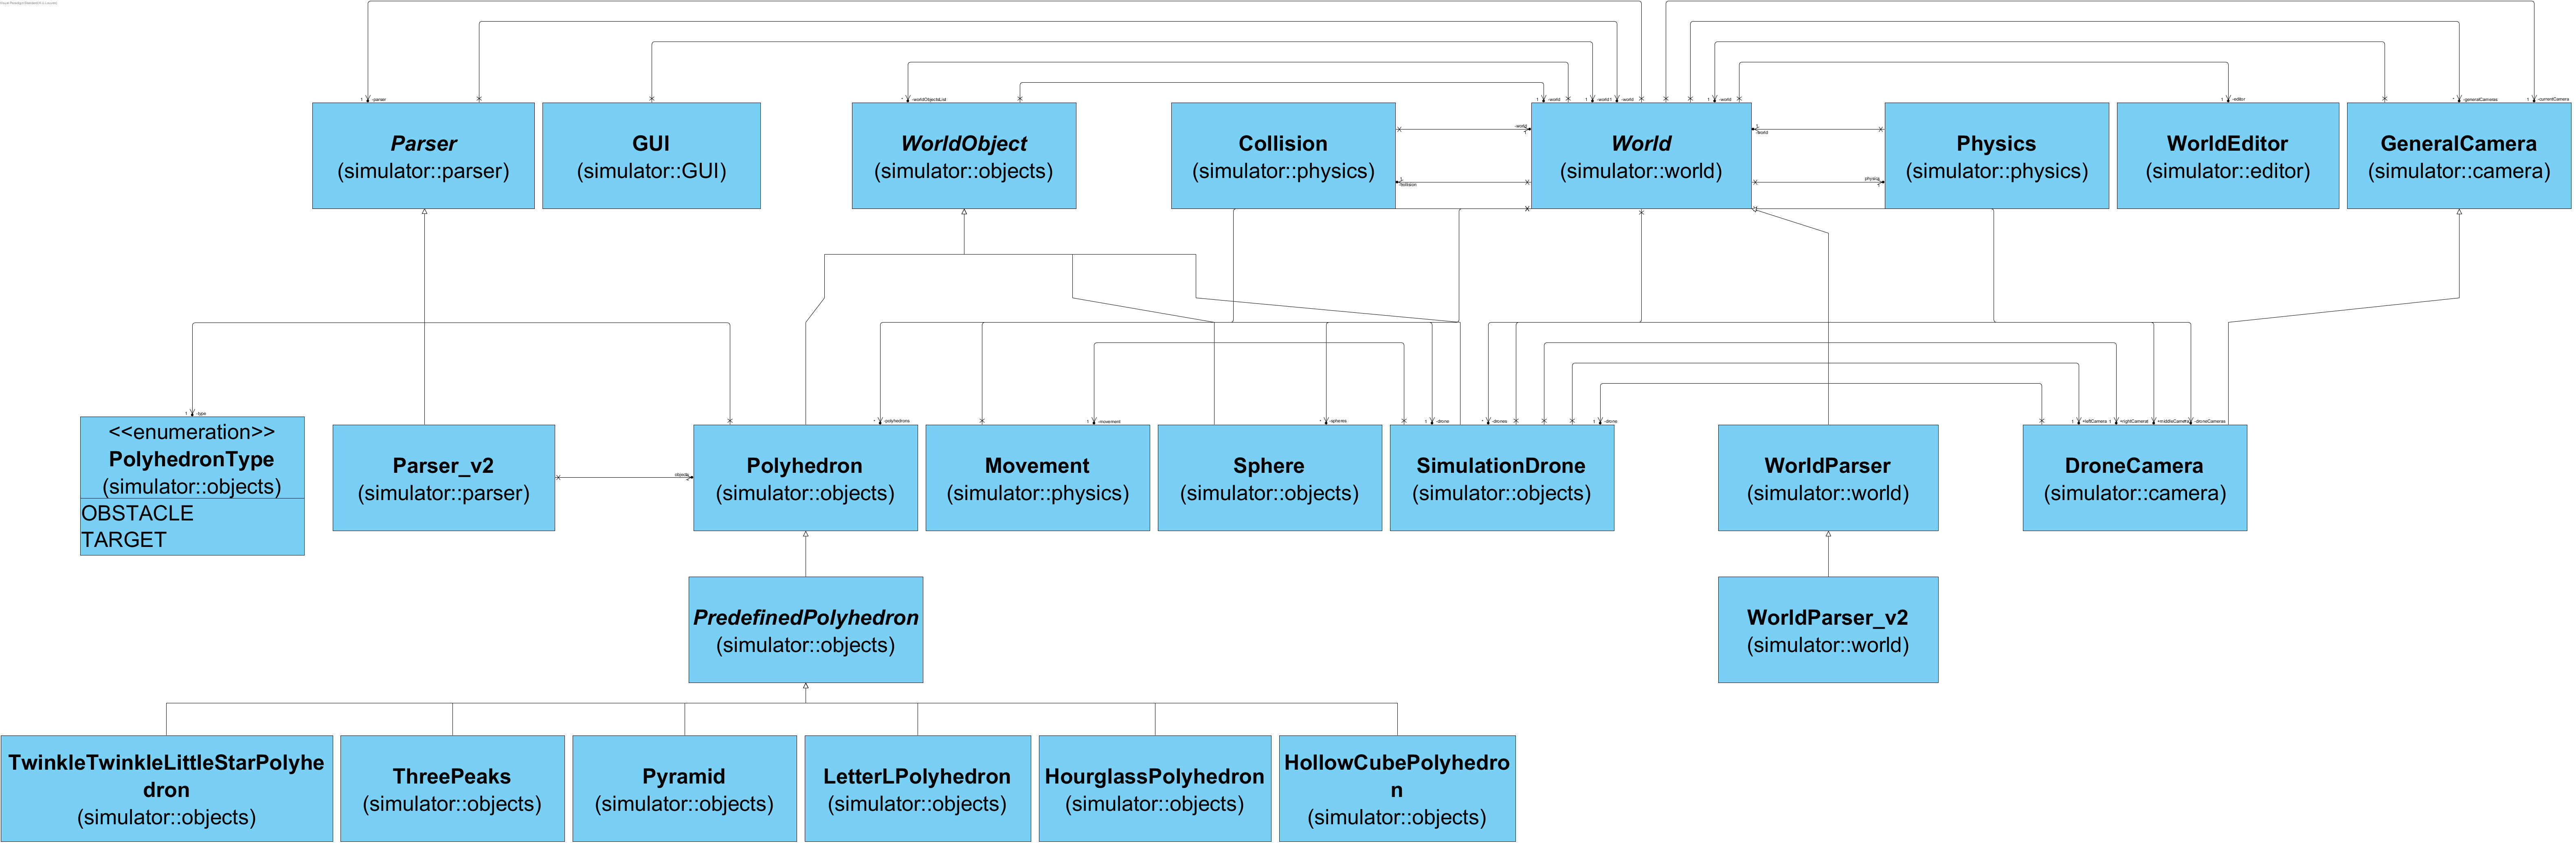
\includegraphics[width=1\linewidth]{Appendices/Simulator.png}
		\end{center}
		\caption{De basisstructuur van het Testbed. Centraal \textit{World}, met de \textit{WorldObjects} (\textit{SimulationDrone}, \textit{Polyhedron}) en enkele hulpklassen. }
\end{figure}
\subsection{Autopilot}
\begin{figure}[H]
		\begin{center}
			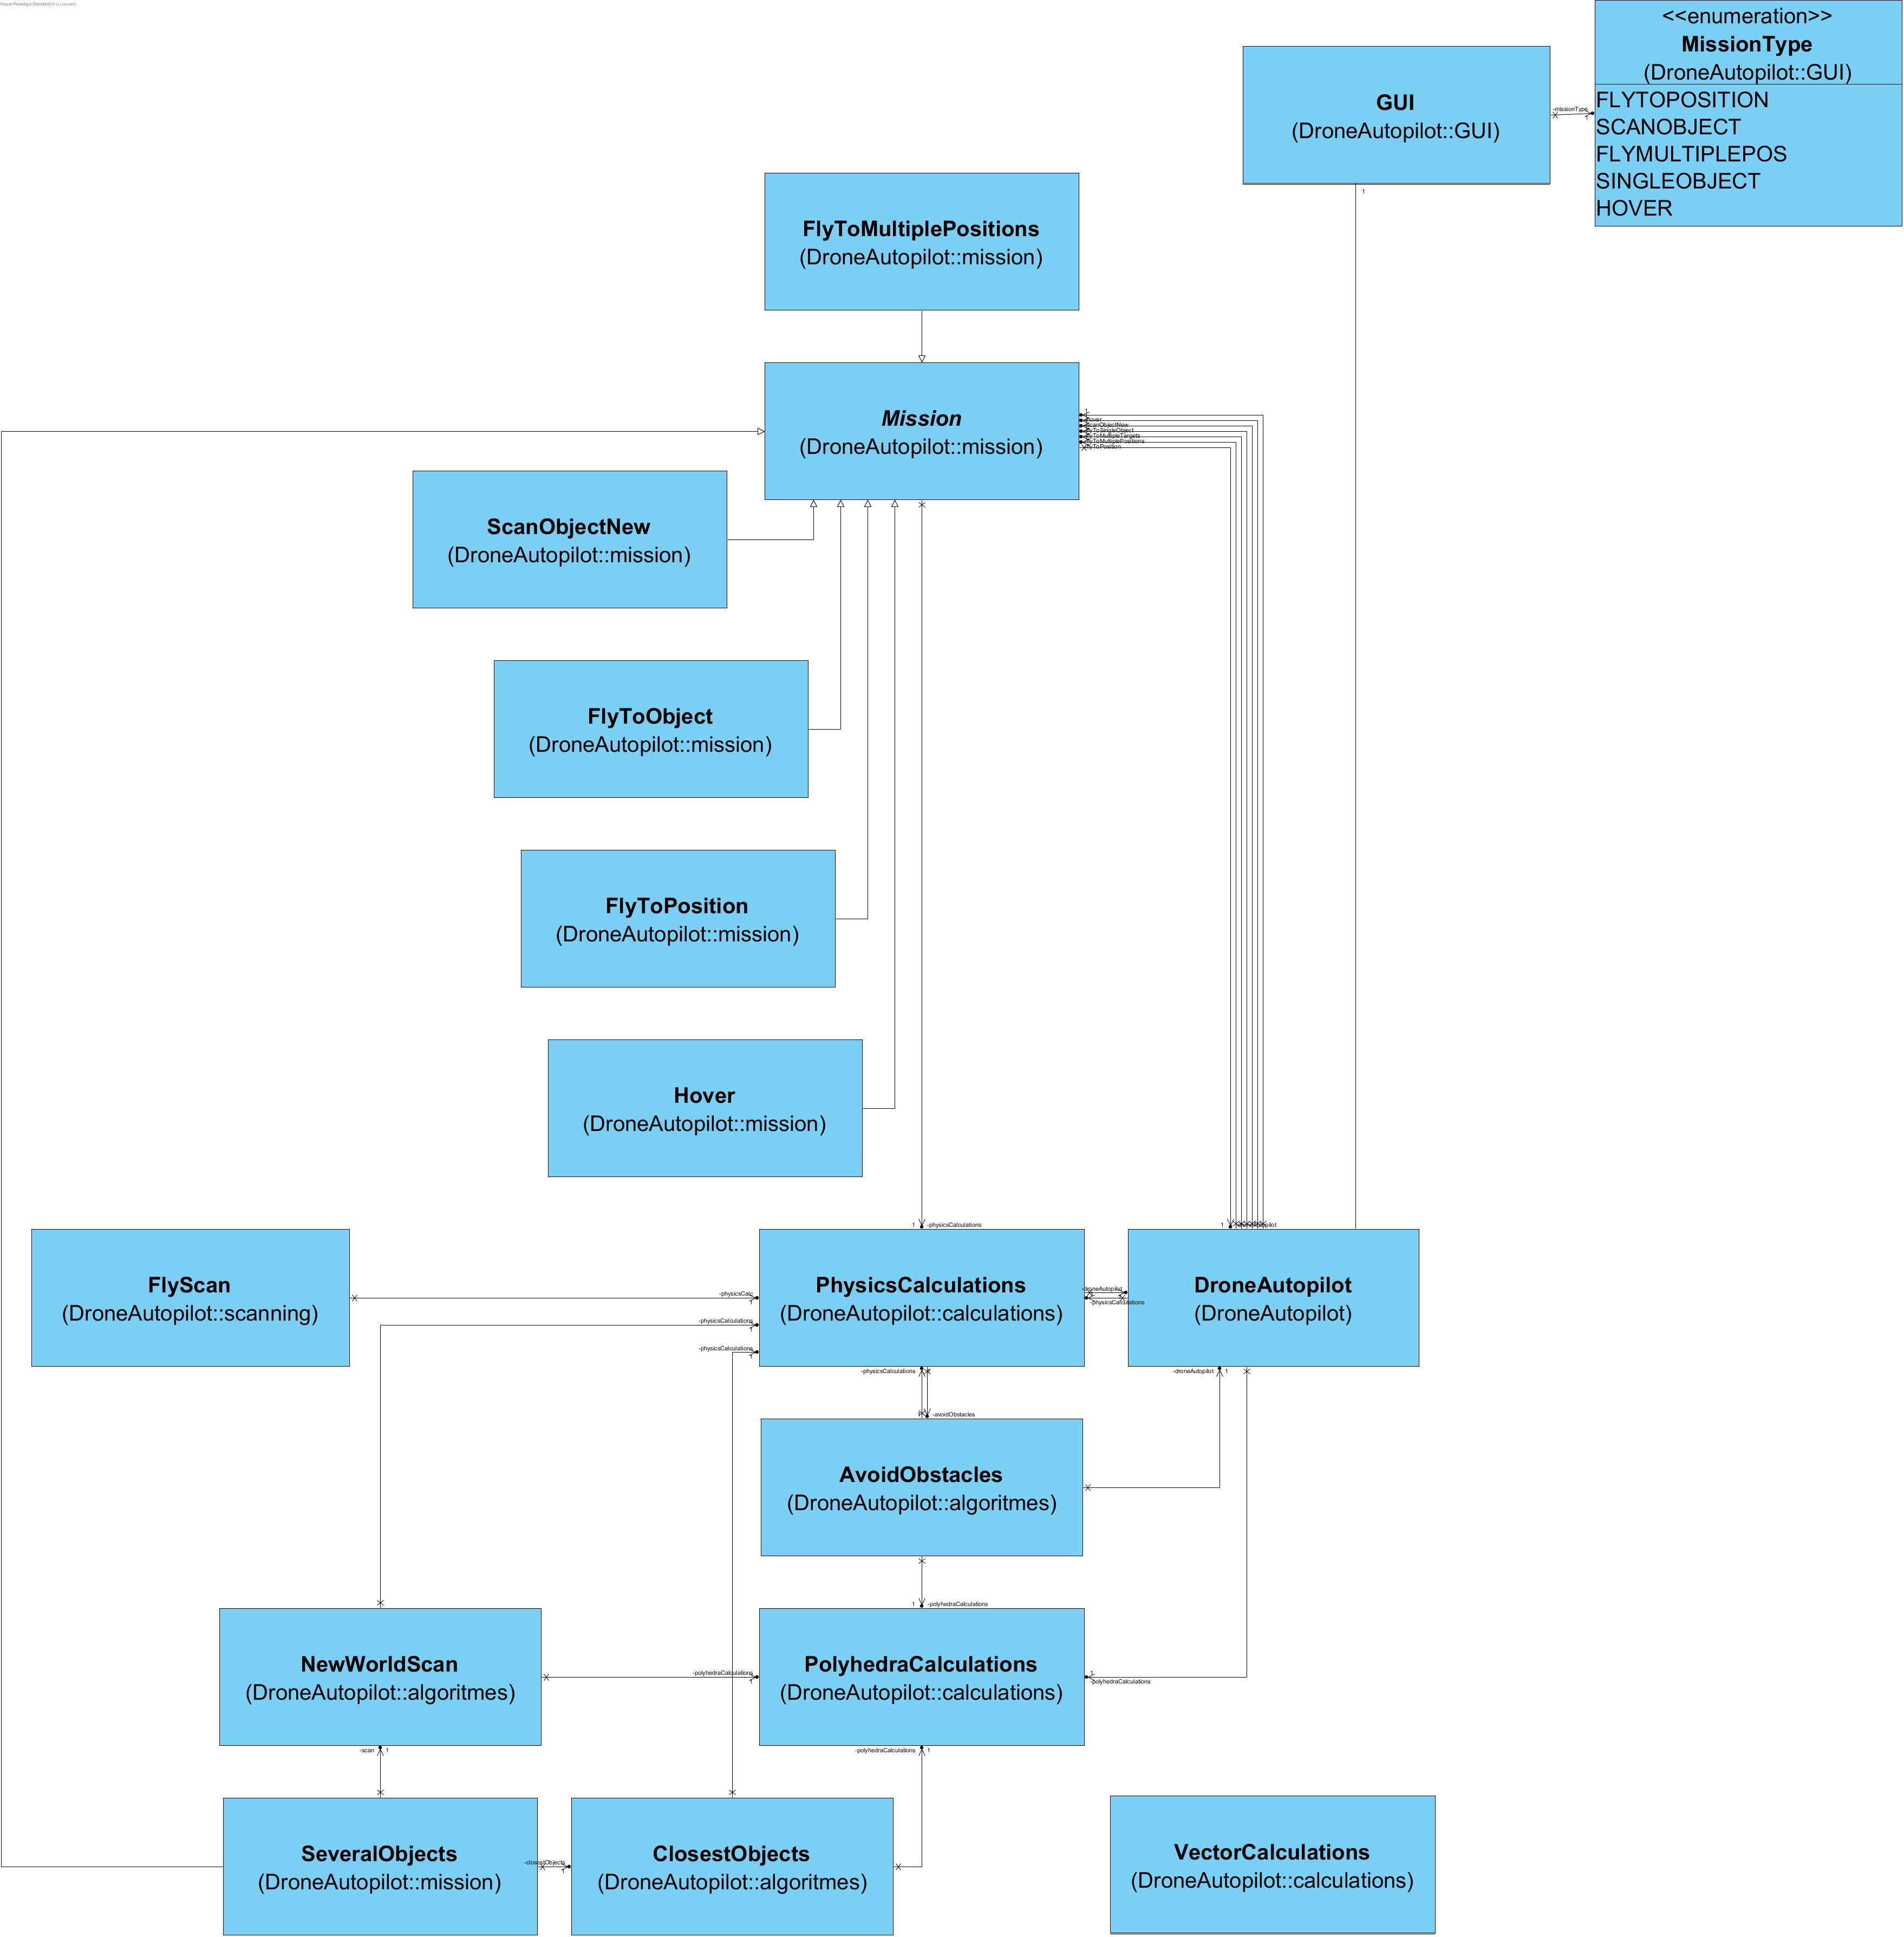
\includegraphics[width=1\linewidth]{Appendices/AP.png}
		\end{center}
		\caption{De basisstructuur weer van de Autopilot. Centrale klassen zijn \textit{Mission, DroneAutopilot} en \textit{PhysicsCalculations}. Dankzij de \textit{Mission}-structuur kon er gemakkelijk opbouwend gewerkt worden en is het duidelijk wat de exacte opdracht van de drone is.}
\end{figure}
\subsection{Scannen}
\begin{figure}[H]
		\begin{center}
			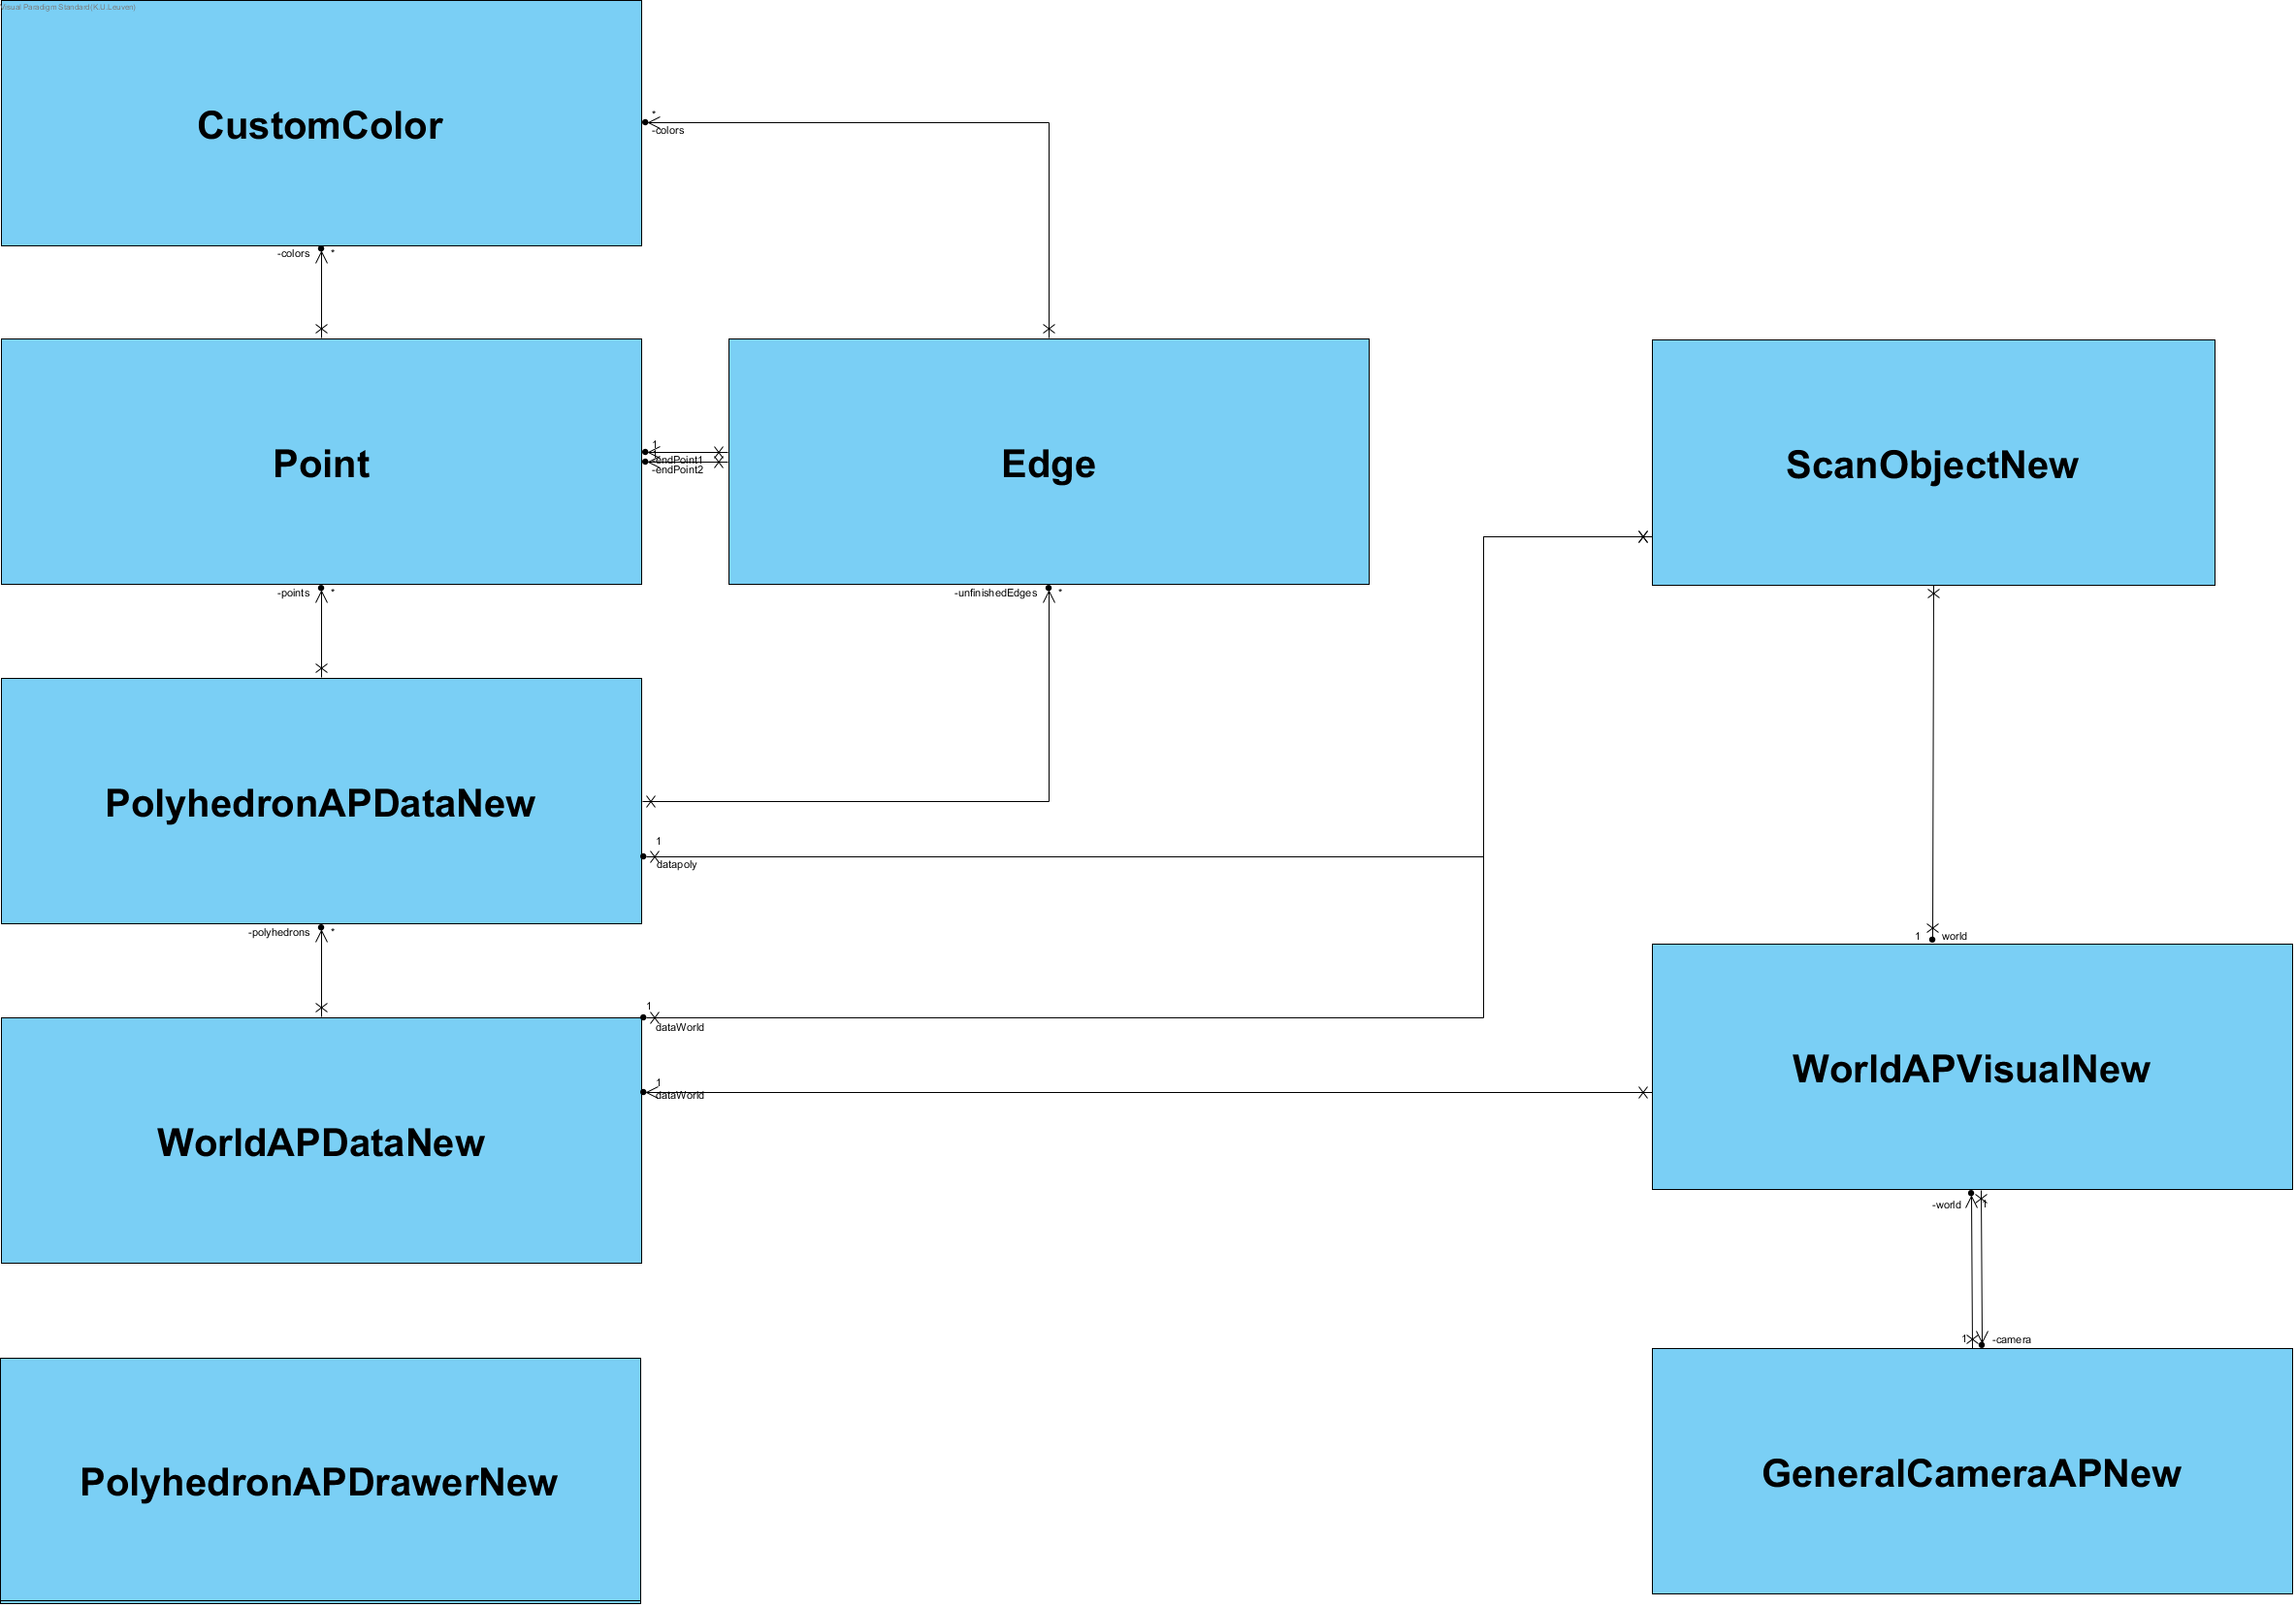
\includegraphics[width=1\linewidth]{Appendices/AP2.png}
		\end{center}
		\caption{De basisstructuur van het scan-gedeelte. Belangrijk zijn de \textit{Polyhedron} en de \textit{WorldAPData} waartoe die behoort. Een \textit{PolyhedronAPData} bestaat uit \textit{Points}, die dan weer \textit{CustomColors} bevatten. }
\end{figure}